\documentclass[class=article]{standalone}
%----------------------------Preamble-------------------------------%
\usepackage{tikz}
%--------------------------Main Document----------------------------%
\begin{document}
    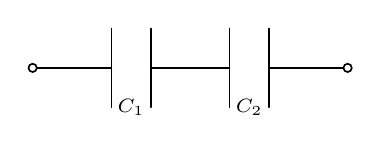
\begin{tikzpicture}[%
        line width=0.6pt,
        line cap=round
    ]
        \begin{scope}[
            every node/.style={
                circle,
                fill=white,
                draw=black,
                inner sep=0pt,
                minimum size=3pt
            }
        ]
            \node (a) at (0,0) {};
            \node (b) at (4,0) {};
        \end{scope}
        \draw (a) to (1,0);
        \draw (1,-0.5) to (1,0.5);
        \draw (1.5,-0.5) to (1.5,0.5);
        \draw (1.5,0) to (2.5,0);
        \draw (2.5,-0.5) to (2.5,0.5);
        \draw (3,-0.5) to (3,0.5);
        \draw (3,0) to (b);
        \node at (1.25,-0.5){\scriptsize{$C_{1}$}};
        \node at (2.75,-0.5){\scriptsize{$C_{2}$}};
    \end{tikzpicture}
\end{document}